% ------------------------------------------------------------------------------
% TYPO3 CMS 8.3 - What's New - Chapter "In-Depth Changes" (English Version)
%
% @author	Patrick Lobacher <patrick@lobacher.de> and Michael Schams <schams.net>
% @license	Creative Commons BY-NC-SA 3.0
% @link		http://typo3.org/download/release-notes/whats-new/
% @language	English
% ------------------------------------------------------------------------------
% LTXE-CHAPTER-UID:		5ebcecbe-66abfa57-cf38bc00-aa637965
% LTXE-CHAPTER-NAME:	In-Depth Changes
% ------------------------------------------------------------------------------

\section{In-Depth Changes}
\begin{frame}[fragile]
	\frametitle{In-Depth Changes}

	\begin{center}\huge{Chapter 3:}\end{center}
	\begin{center}\huge{\color{typo3darkgrey}\textbf{In-Depth Changes}}\end{center}

\end{frame}

% ------------------------------------------------------------------------------
% LTXE-SLIDE-START
% LTXE-SLIDE-UID:		bd33b29d-c20d1765-f923f78e-43bfb0bf
% LTXE-SLIDE-TITLE:		Feature #74365: Add Linkservice for Unified Referencing Syntax (1)
% LTXE-SLIDE-REFERENCE:	Feature-74365-LinkServiceForUnifiedReferencingSyntax.rst
% ------------------------------------------------------------------------------
\begin{frame}[fragile]
	\frametitle{In-Depth Changes}
	\framesubtitle{Add Linkservice for Unified Referencing Syntax (1)}

	\begin{itemize}

		\item Resources within TYPO3 have been referenced using multiple, different forms of syntax in the past.

		\item TYPO3 now supports a modern and future-proof way of referencing resources using an extensible and
			expressive syntax which is easy to understand.

		\item The next slides explain the syntax using the following simple page link:

			\begin{lstlisting}
				t3://page?uid=13&campaignCode=ABC123
			\end{lstlisting}

	\end{itemize}

\end{frame}

% ------------------------------------------------------------------------------
% LTXE-SLIDE-START
% LTXE-SLIDE-UID:		95f9a663-ea2155a1-5635728b-77a8995c
% LTXE-SLIDE-TITLE:		Feature #74365: Add Linkservice for Unified Referencing Syntax (2)
% LTXE-SLIDE-REFERENCE:	Feature-74365-LinkServiceForUnifiedReferencingSyntax.rst
% ------------------------------------------------------------------------------
\begin{frame}[fragile]
	\frametitle{In-Depth Changes}
	\framesubtitle{Add Linkservice for Unified Referencing Syntax (2)}

	\begin{itemize}

		\item The syntax consists of three parts:

			\begin{itemize}

				\item Namespace (\texttt{t3://})\newline
		   			The namespace is fixed to \texttt{t3://} to ensure the "LinkService" is executed to parse the URN.
					\newline
				\item Resource handler key (\texttt{page})\newline
   					The resource handler key identifies the resource in the TYPO3 available handlers list.
					At the time of writing the following handlers exist: \texttt{page}, \texttt{file} and \texttt{folder}.\newline
					More keys can be configured in an associative array, where the key is the handler key and the value
					is a class implementing the LinkHandlerInterface:\newline
					\texttt{\$TYPO3\_CONF\_VARS['SYS']['linkHandler']}

			\end{itemize}

	\end{itemize}

\end{frame}

% ------------------------------------------------------------------------------
% LTXE-SLIDE-START
% LTXE-SLIDE-UID:		77a8995c-ea2155a1-95f9a663-5635728b
% LTXE-SLIDE-TITLE:		Feature #74365: Add Linkservice for Unified Referencing Syntax (3)
% LTXE-SLIDE-REFERENCE:	Feature-74365-LinkServiceForUnifiedReferencingSyntax.rst
% ------------------------------------------------------------------------------
\begin{frame}[fragile]
	\frametitle{In-Depth Changes}
	\framesubtitle{Add Linkservice for Unified Referencing Syntax (3)}

	\begin{itemize}

		\item ...and the 3rd part:

			\begin{itemize}

				\item Resource parameters (\texttt{?uid=13\&campaignCode=ABC123})\newline
					These are the specific identification parameters that are used by any handler.
					Note that these may carry additional parameters in order to configure the behavior of any handler.

			\end{itemize}

	\end{itemize}

\end{frame}

% ------------------------------------------------------------------------------
% LTXE-SLIDE-START
% LTXE-SLIDE-UID:		af8e73a4-2b315873-bb6e55e4-c0cd82b5
% LTXE-SLIDE-TITLE:		#76008 and #76458: DebuggerUtility::var_dump (1)
% LTXE-SLIDE-REFERENCE:	Feature-76008-PropertyVisibilityToDebuggerUtilityvar_dump.rst
% LTXE-SLIDE-REFERENCE:	Feature-76458-LetDebuggerUtilityRenderClosures.rst
% ------------------------------------------------------------------------------
\begin{frame}[fragile]
	\frametitle{In-Depth Changes}
	\framesubtitle{\texttt{DebuggerUtility::var\_dump} (1)}

	\begin{itemize}

		\item The property visibility information has been added to \texttt{DebuggerUtility::var\_dump()}
			\newline
			for each object property in the dump

		\item If a closure is part of the debugging object, the source code of the closure is rendered, too

	\end{itemize}

	\tabto{0.75cm}\textit{See example on the next slide}

\end{frame}

% ------------------------------------------------------------------------------
% LTXE-SLIDE-START
% LTXE-SLIDE-UID:		bb6e55e4-2b315873-c0cd82b5-af8e73a4
% LTXE-SLIDE-TITLE:		#76008 and #76458: DebuggerUtility::var_dump (2)
% LTXE-SLIDE-REFERENCE:	Feature-76008-PropertyVisibilityToDebuggerUtilityvar_dump.rst
% LTXE-SLIDE-REFERENCE:	Feature-76458-LetDebuggerUtilityRenderClosures.rst
% ------------------------------------------------------------------------------
\begin{frame}[fragile]
	\frametitle{In-Depth Changes}
	\framesubtitle{\texttt{DebuggerUtility::var\_dump} (2)}

	\begin{figure}
		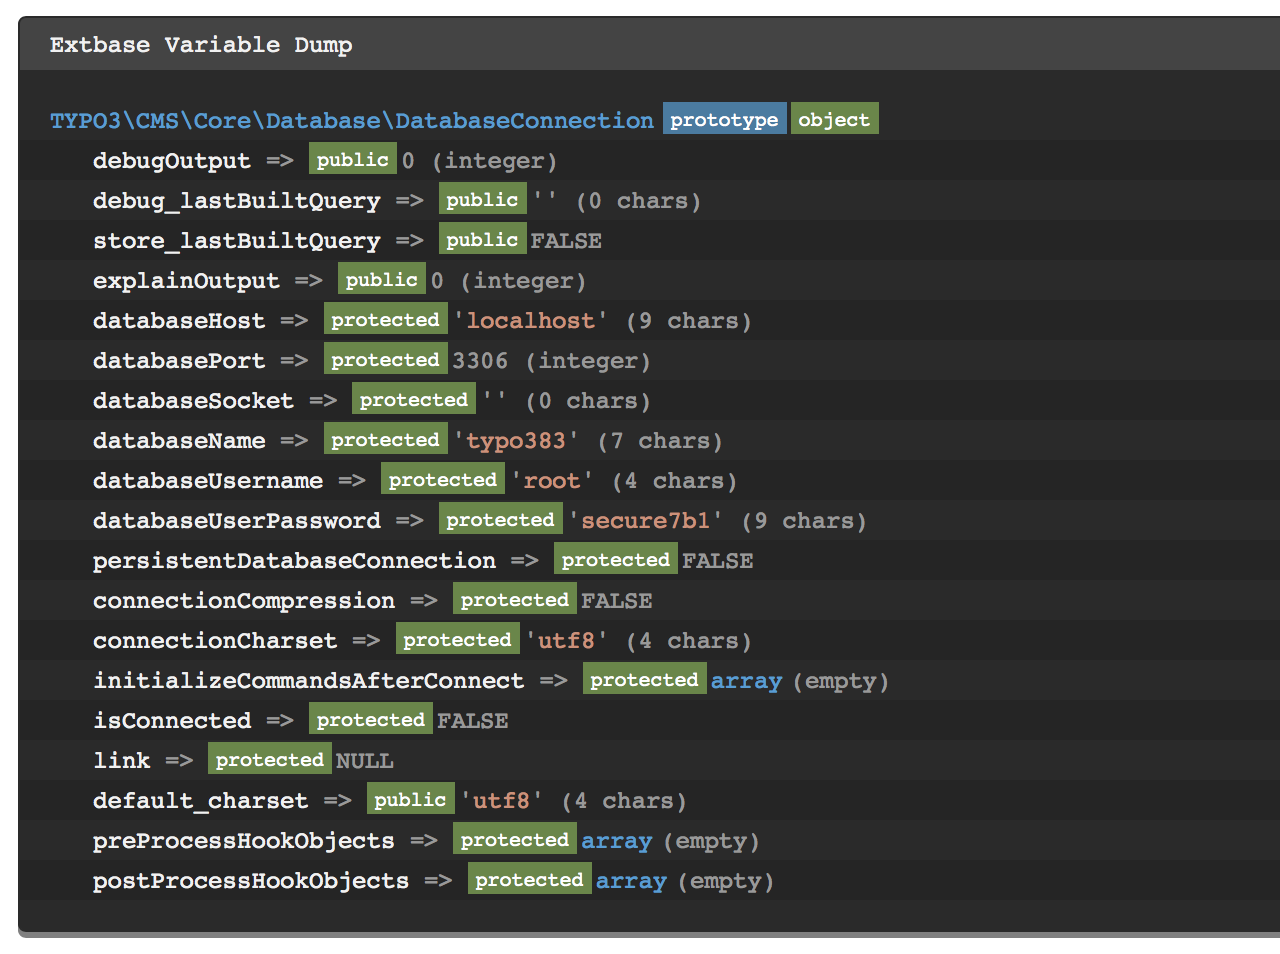
\includegraphics[width=0.65\linewidth]{InDepthChanges/76008.png}
	\end{figure}

\end{frame}

% ------------------------------------------------------------------------------
% LTXE-SLIDE-START
% LTXE-SLIDE-UID:		2b74180d-e68ba0c2-8826a2cf-8498f977
% LTXE-SLIDE-TITLE:		!Breaking: #73461 - Import module disabled for non admin users
% LTXE-SLIDE-REFERENCE:	!Breaking-73461-ImportModuleDisabledForNonAdminUsers.rst
% ------------------------------------------------------------------------------
\begin{frame}[fragile]
	\frametitle{In-Depth Changes}
	\framesubtitle{Import Module Disabled for Non Admin Users}

	\begin{itemize}

		\item The import module of \texttt{EXT:impexp} is now disabled for non-admin users by default

		\item For non-admin users, who need that functionality, the following User TSconfig option
			can be set:\newline
			\texttt{options.impexp.enableImportForNonAdminUser = 1}

			\vspace{0.5cm}

			\begingroup
				\color{typo3red}
				Warning: this can become a security problem in TYPO3 versions 6.2 and 7.6
				and should only be enabled for \textit{trustworthy} backend users.
			\endgroup

	\end{itemize}

\end{frame}

% ------------------------------------------------------------------------------
% LTXE-SLIDE-START
% LTXE-SLIDE-UID:		bac423cc-ba00db30-e1538b7f-25749380
% LTXE-SLIDE-TITLE:		Hooks and Signals (1)
% LTXE-SLIDE-REFERENCE:	!Feature-76209-HookToRegisterCustomResultBrowsersInAbstractPlugin.rst
% ------------------------------------------------------------------------------
\begin{frame}[fragile]
	\frametitle{In-Depth Changes}
	\framesubtitle{Hooks and Signals (1)}

	% decrease font size for code listing
	\lstset{basicstyle=\tiny\ttfamily}

	\begin{itemize}

		\item A new hook allows registering custom result browser implementations

		\item This approach allows to override the default implementation of
			\texttt{AbstractPlugin::pi\_list\_browseresults()}
			for either all extensions or only for specific ones

		\item The hook can be registered in \texttt{ext\_localconf.php}:

			\begin{lstlisting}
				$GLOBALS['TYPO3_CONF_VARS']['SC_OPTIONS']
				  [\TYPO3\CMS\Frontend\Plugin\AbstractPlugin::class]['pi_list_browseresults'][1463475262] =
				  \Vendor\ExtensionKey\Hook\ResultBrowserHook::class
			\end{lstlisting}

	\end{itemize}

\end{frame}


% ------------------------------------------------------------------------------
% LTXE-SLIDE-START
% LTXE-SLIDE-UID:		82c70aee-3b375252-6cac0ad6-b385b95f
% LTXE-SLIDE-TITLE:		Hooks and Signals (2)
% LTXE-SLIDE-REFERENCE:	!Feature-76259-IntroduceBuildQueryParametersPostProcessHook.rst
% ------------------------------------------------------------------------------
\begin{frame}[fragile]
	\frametitle{In-Depth Changes}
	\framesubtitle{Hooks and Signals (2)}

	% decrease font size for code listing
	\lstset{basicstyle=\tiny\ttfamily}

	\begin{itemize}

		\item With the migration to Doctrine, hook \texttt{buildQueryParameters} has been introduced in class
			\texttt{DatabaseRecordList}.

		\item This hook replaces the hook \texttt{makeQueryArray} from the deprecated method
			\texttt{AbstractDatabaseRecordList::makeQueryArray}.

		\item Using the new hook allows modifying the parameters used to query the database for records
			to be shown in the record list view

		\item The hook can be registered in \texttt{ext\_localconf.php}:

			\begin{lstlisting}
				$GLOBALS['TYPO3_CONF_VARS']['SC_OPTIONS']
				  [\TYPO3\CMS\Recordlist\RecordList\DatabaseRecordList::class]['buildQueryParameters'][]
			\end{lstlisting}

		\item ...and implements the public method \texttt{buildQueryParametersPostProcess}

	\end{itemize}

\end{frame}

% ------------------------------------------------------------------------------
% LTXE-SLIDE-START
% LTXE-SLIDE-UID:		73d888ce-a14c0f6a-d4dec5fb-f7368bb6
% LTXE-SLIDE-TITLE:		!Breaking: #76108 - Replace ExtJS category tree with D3 and SVG
% LTXE-SLIDE-TITLE:		!Feature: #77349 - Additional locations for extension icons
% LTXE-SLIDE-TITLE:		!Feature: #77481 - Add possibility to define a favicon for the backend
% LTXE-SLIDE-REFERENCE:	!Breaking-76108-ReplaceExtJSCategoryTreeWithD3AndSVG.rst
% LTXE-SLIDE-REFERENCE:	!Feature-77349-AdditionalLocationsForExtensionIcons.rst
% LTXE-SLIDE-REFERENCE:	!Feature-77481-AddPossibilityToDefineAFaviconForTheBackend.rst
% ------------------------------------------------------------------------------
\begin{frame}[fragile]
	\frametitle{In-Depth Changes}
	\framesubtitle{Miscellaneous}

	\begin{itemize}

		\item SVGs and D3 rendering

			\begin{itemize}
				\item As part of the ExtJS removal from the TYPO3 core, the tree within the form editing has been re-worked
				\item Rendering is based on SVGs and D3 now, which comes with a significant performance boost
				\item Re-working the page tree the same way is planned for the near future
			\end{itemize}

		\item Extension icons can be stored in the following directory now:\newline
			\small
				\texttt{Resources/Public/Icons/<filename>}
				(where <filename> can be: \texttt{Extension.png}, \texttt{Extension.svg} or \texttt{Extension.gif})
			\normalsize

		\item The new option \texttt{backendFavicon} in the Extension Manager configuration makes it possible to
			change the favicon of the backend.

	\end{itemize}

\end{frame}

% ------------------------------------------------------------------------------
